\documentclass[a4paper]{article} % default is 10 pt
\usepackage{graphicx} % needed for including graphics e.g. EPS, PS
\usepackage{gensymb}
\usepackage{titling}
\usepackage{array}
\usepackage{subfig}
\usepackage{listings}
%\usepackage{amsmath}
%\usepackage[]{algorithm2e}
%\usepackage{algorithm}
%\usepackage{algpseudocode}
\usepackage[numbers]{natbib}

\newcommand{\subtitle}[1]{%
  \posttitle{%
    \par\end{center}
    \begin{center}\large#1\end{center}
    \vskip0.5em}%
}

\long\def\comment#1{}

\captionsetup[table]{belowskip = 12pt, aboveskip = 4pt}
% uncomment if you don't want page numbers
% \pagestyle{empty}

%set dimensions of columns, gap between columns, and paragraph indent 
\setlength{\textheight}{8.75in}
\setlength{\columnsep}{0.375in}
\setlength{\textwidth}{6.8in}
\setlength{\topmargin}{0.0625in}
\setlength{\headheight}{0.0in}
\setlength{\headsep}{0.0in}
\setlength{\oddsidemargin}{-.19in}
\setlength{\parindent}{0pt}
\setlength{\parskip}{0.12in}
\makeatletter
\def\@normalsize{\@setsize\normalsize{10pt}\xpt\@xpt
  \abovedisplayskip 10pt plus2pt minus5pt\belowdisplayskip 
  \abovedisplayskip \abovedisplayshortskip \z@ 
  plus3pt\belowdisplayshortskip 6pt plus3pt 
  minus3pt\let\@listi\@listI}

%need an 11 pt font size for subsection and abstract headings 
\def\subsize{\@setsize\subsize{12pt}\xipt\@xipt}
%make section titles bold and 12 point, 2 blank lines before, 1 after
\def\section{\@startsection {section}{1}{\z@}{1.0ex plus
    1ex minus .2ex}{.2ex plus .2ex}{\large\bf}}
%make subsection titles bold and 11 point, 1 blank line before, 1 after
\def\subsection{\@startsection 
  {subsection}{2}{\z@}{.2ex plus 1ex} {.2ex plus .2ex}{\subsize\bf}}
\makeatother



\begin{document}

% don't want date printed
\date{}

% >>>>>>>>>>>>>>>>>>>>>>>  Put your title here <<<<<<<<<<<<<<<<<<<<<<<<
% make title bold and 14 pt font (Latex default is non-bold, 16pt) 
\title{\Large {\bf Assignment Report - 3 (Revised Version 2)} }
\subtitle{\bf Green's Boundary Integral Method for a Cylindrical Heaving Buoy \vspace{-4ex}}
% >>>>>>>>>>>>>>>>>>>>>>> Author's Name, Thanks or Affiliation <<<<<<<<
\author{Aditya Narayanan (OE13S013)
  \thanks{email: adityarn@gmail.com
  }
}
\maketitle \vspace{-12ex}
\thispagestyle{empty}

\subsection*{\centering Abstract}

% >>>>>>>>>>>>>>>>>>>>>>>>> Keywords and Abstract <<<<<<<<<<<<<<<<<<<<<
% Replace with your own keywords and abstract.  Text will be in italics
{
Green's boundary integral method or panel method is used to obtain the added mass and radiation damping of a heaving cylinder in a small amplitude wave regime.
}

% >>>>>>>>>>>>>>>>>>>>>> START OF YOUR PAPER <<<<<<<<<<<<<<<<<<<<<<<<<<<<<<

\section{Problem Statement}
Using the frequency-domain boundary integral method with $ G = \frac{1}{r} $ numerically solve the heave radiation problem of a vertical circular cylinder.

\begin{enumerate}

\item Cylinder diameter, D = 1 m
\item Cylinder draft, d = 3 m
\item Water depth, h = 10 m
\item Water depth, h = 10 m
\item Frequency, $\sigma$ from 0.1 to 5 [rad/s]

\end{enumerate}

and also compute the heave added-mass $\mu_{zz}$ and damping $\lambda_{zz}$ with total number of panels N=5000 and 10000.

\section{Formulation}
Since the cylinder is small compared to the incident wave's wavelength ($D/L << 1$), we neglect the scattering wave potential in this solution. We treat this
as a linear problem, ie. it is assumed that the wave has a small enough amplitude to neglect non-linearities, which allows us to decompose the total
fluid potential into separate components.

$$ \phi = \phi^i + \phi^r $$

The radiation potential must satisfy the following:
$$\nabla^2 \Phi^r = 0 \mbox{,     in   } \forall $$ 
We apply the boundary conditions for the radiation potential at the body surface:
$$ \frac{\partial \Phi^r}{\partial n} = V_n $$
$$\mbox{where, } V_n = \vec U . \hat n + \vec \ohm . (\vec r \times \hat n) $$

The free surface boundary condition applied is:
$$ \frac{\partial^2 \Phi^r}{\partial t^2} + g\frac{\partial \Phi^r}{\partial z} = 0 \mbox{,  on } z=0 $$

The radiation potential can be computed in the frequency domain by separating the time function:
$$ \Phi^r = \sum_{j=1}^{6} \phi^r_j = e^{-i\sigma t} \sum_{j=1}^{6} \varphi^r_j$$

If we define a displacement $\xi_j$ as the displacement due to the $j^{th}$ mode of oscillation, then:
$$\xi_j = A_j e^{-i\sigma t} $$
The velocity and acceleration would then be:
$$ \frac{d \xi_j}{dt} = -i\sigma t A_j e^{-i\sigma t} $$
$$ \frac{d^2 \xi_j}{dt^2} = -\sigma^2 t A_j e^{-i\sigma t} $$

The radiation potential can be represented per unit displacement, as:
$$ \varphi_j^r = A_j \psi_j^r $$
This radiation potential satisfies the following conditions:
$$\nabla^2 \psi_j^r = 0 \mbox{,     in   } \forall $$ 
$$\nabla \psi_j^r \rightarrow 0 \mbox{,   as  } z \rightarrow -\infty $$

Free surface condition:
$$ -\sigma^2 \psi_j^r + g \frac{\partial \psi_j^r}{\partial z} = 0 \mbox{,   on   } z=0 $$

Sommerfeld radiation condition:
$$ -i\sigma \psi_j^r + \frac{\sigma}{K} \frac{\partial \psi_j^r}{\partial R} = 0 \mbox{,   at  } R \rightarrow \infty $$

The force on the body, (obtained by integrating the dynamic pressure over the body surface):
$$ F_{jk} = -\big[ -\sigma^2 A_j e^{-i\sigma t} \mu_{jk} - i\sigma A_j e^{-i\sigma t} \lambda_{jk} \big] $$

The force per unit amplitude and in frequency domain will be:
$$ f_{jk} = -\sigma^2 \mu_{jk} - i\sigma \lambda_{jk} $$
where,
$$ f_{jk} = \rho \int_{S_0} \psi_j^r \frac{\partial \psi_k^r}{\partial n} dS_0 $$
$$ \mu_{jk} = \frac{\mbox{Real}(f_{jk})}{-\sigma^2} \mbox{   and   } \lambda_{jk} = \frac{Imag(f_{jk})}{-\sigma} $$ 


%**********************************************************************************************************************

\section{Methodology}
The Green's mixed distribution method is used, and by using the appropriate boundary conditions for the radiation potential, we get the following

\begin{eqnarray}
2 \pi \varphi(P) + \int_{S_0} \varphi \Big( \frac{\partial}{\partial n}\frac{1}{r} dS_0 \Big) &+& 
 \int_{F_0} { \varphi \Big(\frac{\partial}{\partial n}\frac{1}{r} - \frac{1}{r} \frac{\sigma^2}{g} \Big) dF_0}
 + \int_B \varphi \Big(\frac{\partial}{\partial n} \frac{1}{r} \Big) dB \nonumber \\
&+& \int_{\Sigma} \varphi \Big(\frac{\partial}{\partial n} \frac{1}{r} - \frac{1}{r}ik \Big) d\Sigma \  = \int_{S_0} \frac{1}{r}V_n dS_0
\label{GMD}
\end{eqnarray}

Where, $S_0$ is the body's surface, $F_0$ is the free surface, $B$ is the bottom surface, and $\Sigma$ is the far-field surface.

For the j'th mode of operation, $$V_n = \frac{\partial \varphi_j^r}{\partial n} = -i\sigma n_j $$

The above system of equations can be represented as:
$$ C_{ij} \varphi_j = b_j $$

The system when solved gives us the radiation potential at each panel on all the four surfaces. The forces when integrated over the surface of the 
oscillating body (using the potentials obtained by solving the equations) give us the added mass and damping.

The mesh used in the solution is shown in fig \ref{mesh}.

\begin{figure*}[h]
\centering
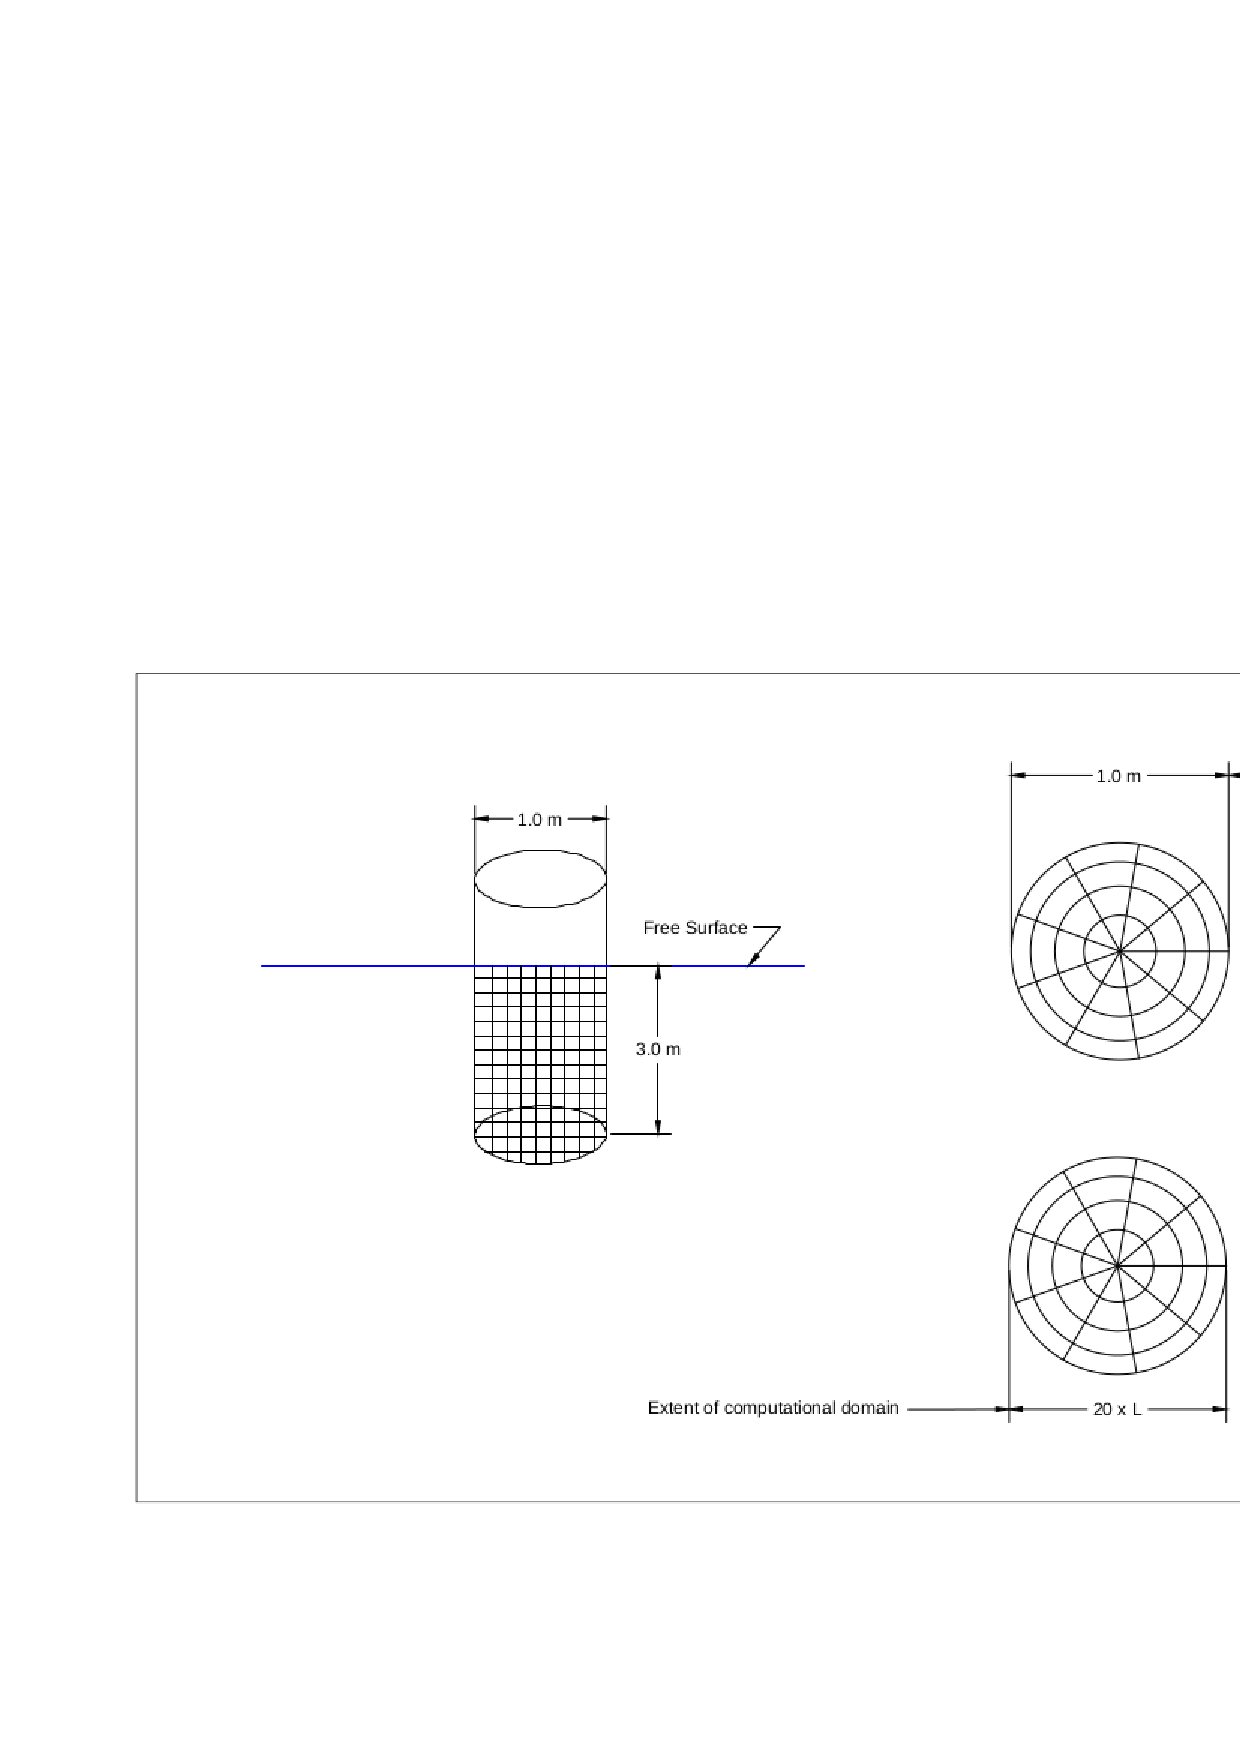
\includegraphics[width=140mm]{mesh}
\caption{Mesh for cylinder, free surface, far-field, and bottom surface}
\label{mesh}
\end{figure*}

\pagebreak
\section{Results}
The table shows the final results obtained. As is evident, the damping is very low, and the added mass is about 1.02 to 1.03.
$$ (\mbox{Mass displaced by buoy}) = \rho \times \pi \times 1^2 \times 3.0 = 9660.4 Kg $$
$$ \mbox{Added Mass coefficient}, C_a = \frac{(\mbox{added mass})}{\mbox{(added mass + mass displaced)}} $$

\begin{table}[htbp]
\centering
\caption{Results - Mu and Damping coefficients in a non-dimensionalized form}
\begin{tabular}{|r|r|r|r|r|}
\hline
\multicolumn{1}{|c|}{\textbf{Total no of panels}} & \multicolumn{1}{c|}{\textbf{no of body panels}} & \multicolumn{1}{c|}{\textbf{Sigma}} & \multicolumn{1}{c|}{\textbf{Mu}} & \multicolumn{1}{c|}{\textbf{Damping}} \\ \hline
6191 & 1250 & 0.628 & 1.0306243785 & 1.0000068937 \\ \hline
6191 & 1250 & 5 & 1.0249887263 & 1.0000433711 \\ \hline
\end{tabular}
\label{results_table}
\end{table}


\pagebreak
\section{Program Listing}

\subsection{C++ Program to Generate Coordinates}
\lstinputlisting[breaklines=true]{proj3_coord_gen.cpp}

\subsection{Python Code to Solve the Green's Mixed Distribution Equations}

\begin{lstlisting}[language=Python, breaklines=true]
import numpy as np
import linecache

'''Reading From Input File "xyz.txt"
which contains all coordinates, normals
and area of each panel. This file is
generated with the C++ code "coord_gen.cpp" '''

c = 0
line = linecache.getline("xyz.txt",c+1)
line_arr = line.split()

Time_period = float(line_arr[0])
L = float(line_arr[1])
n_total = int(line_arr[2])
n_body = int(line_arr[3])
n_fs = int(line_arr[4])
n_bottom = int(line_arr[5])
n_ff = int(line_arr[6])

Kl = 2*np.pi/L
sigma = 2*np.pi/Time_period

x = np.zeros(n_total)
y = np.zeros(n_total)
z = np.zeros(n_total)
nx = np.zeros(n_total)
ny = np.zeros(n_total)
nz = np.zeros(n_total)
ar = np.zeros(n_total)
a = np.zeros((n_total,n_total),dtype=complex)
b = np.zeros(n_total,dtype=complex)
phi = np.zeros(n_total,dtype=complex)

for c in range(n_total):
    line = linecache.getline("xyz.txt",c+2)
    line_arr = line.split()
    x[c] = float(line_arr[0])
    y[c] = float(line_arr[1])
    z[c] = float(line_arr[2])
    nx[c] = float(line_arr[3])
    ny[c] = float(line_arr[4])
    nz[c] = float(line_arr[5])
    ar[c] = float(line_arr[6])

'''Green's mixed Distribution coefficients and RHS matrix are 
computed here'''
for i in range(n_total):
    for k in range(n_body):
        if(i!=k):
            r = (x[i]-x[k])**2 + (y[i]-y[k])**2 + (z[i]-z[k])**2
            numer = -sigma * nz[k]* ar[k]
            denom = r**0.5
            b[i] += complex(0,numer/denom)

    for k in range(n_body):
        if(i != k):
            r = (x[i]-x[k])**2 + (y[i]-y[k])**2 + (z[i]-z[k])**2
            numer = ((x[i]-x[k])*nx[k] + (y[i]-y[k])*ny[k] + (z[i]-z[k])*nz[k])*ar[k]
            denom = r**1.5
            a[i][k] = complex(numer/denom,0)
        else:
            a[i][k] = complex(2*np.pi,0)
    
    for k in range(n_body,n_body+n_fs,1):
        if(i != k):
            r = (x[i]-x[k])**2 + (y[i]-y[k])**2 + (z[i]-z[k])**2
            numer = (x[i]-x[k])*nx[k] + (y[i]-y[k])*ny[k] + (z[i]-z[k])*nz[k]
            denom = r**1.5
            numer2 = sigma**2
            denom2 = 9.81 * r**0.5
            a[i][k] = complex((numer/denom - numer2/denom2)*ar[k],0)
        else:
            a[i][k] = complex(2*np.pi,0)

    for k in range(n_body+n_fs,n_body+n_fs+n_bottom,1):
        if(i != k):
            r = (x[i]-x[k])**2 + (y[i]-y[k])**2 + (z[i]-z[k])**2
            numer = ((x[i]-x[k])*nx[k] + (y[i]-y[k])*ny[k] + (z[i]-z[k])*nz[k])*ar[k]
            denom = r**1.5
            a[i][k] = complex(numer/denom,0)
        else:
            a[i][k] = complex(2*np.pi,0)
            
    for k in range(n_body+n_fs+n_bottom,n_total,1):
        if(i != k):
            r = (x[i]-x[k])**2 + (y[i]-y[k])**2 + (z[i]-z[k])**2
            numer = ((x[i]-x[k])*nx[k] + (y[i]-y[k])*ny[k] + (z[i]-z[k])*nz[k])*ar[k]
            denom = r**1.5
            numer2 = Kl/r
            a[i][k] = complex((numer/denom*ar[k]), -numer2*ar[k])
        else:
            a[i][k] = 2*np.pi

phi = np.linalg.solve(a,b)

fjk = complex(0.0,0.0)
for i in range(n_body):
    fjk +=  phi[i] * nz[i] * ar[i]

fjk = fjk * 1025. * sigma * complex(0,-1)

mu = fjk.real /(-sigma**2)
damping = fjk.imag/(-sigma)

\end{lstlisting}

\end{document}
